\documentclass[11pt,a4paper]{article}
\usepackage{graphicx}
\graphicspath{{img/}}
\usepackage{caption}
\usepackage{subcaption}
\usepackage[utf8]{inputenc}
\usepackage{amsmath}
\usepackage{amsfonts}
\usepackage{easy-todo}
\usepackage{amssymb}
\usepackage[left=3cm,right=3cm,top=3cm,bottom=4cm]{geometry}
\usepackage[colorlinks,linkcolor=black,citecolor=black,filecolor=black]{hyperref}
\usepackage{listings}

% ---- Bibliography -----
\usepackage[style=numeric,bibstyle=numeric,backend=bibtex,sorting=none,maxbibnames=99]{biblatex}
\renewcommand*{\multinamedelim}{;~}
\renewcommand*{\finalnamedelim}{~and~}
\renewcommand*{\mkbibnamelast}[1]{\textsc{#1}}
\DeclareNameAlias{default}{last-first}
\DeclareFieldFormat[article,inbook,incollection,inproceedings,patent,thesis,unpublished]{title}{\textit{#1\isdot}}
\bibliography{bibli.bib}

\catcode`^=\active
\def^#1^{\texttt{#1}}

\begin{document}
\title{Autonomous Agents - Assignment 3}
\author{Bas Veeling (10767770) \and Sebastian Droeppelmann (5783453) \and Fritjof Buettner (10876782)}
\maketitle
\begin{figure}[h!]
	\centering
    \frame{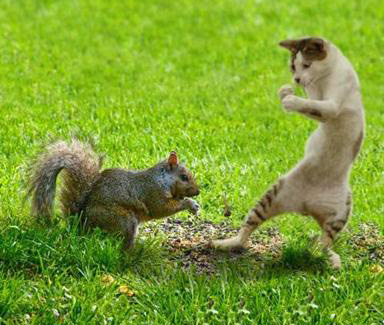
\includegraphics[width=0.5\textwidth]{squirrel}}
   \label{fig:squirrel}
\end{figure}

\section{Introduction}
The focus in this assignment lies in Multi-Agent Planning and learning algorithms.

We have implemented Independent Q-learning and Independent Sarsa as two naive learning algorithms. We then move to more sophisticated algorithms: Minimax-Q and WoLF Policy Hill Climbing.
\section{Multi-agent environment}

% Briefly discuss changes in the implementation
\subsection{Implementation}
The changes to the game for this assignment introduced some alterations to our implementation. These will be briefly discussed in this subsection.
    % New statespace
\paragraph*{State Representation}
Allowing for multiple predators meant altering the state representation. Instead of representing the state with the relative distance from the predator to the prey, it is now represented as an ordered list of these relative distances for every predator to the prey. This does mean that we allow for only one Prey in our implementation.
    % Tripping
\paragraph*{Tripping}
Tripping is implemented in the ^Field^ class' ^transition^ function. Each ^player^ subclass has a tripping probability: 0.2 for the prey, and 0 for the predator. This allows us to experiment with different values. For example, a tripping probability of 1 implies a player is stuck, which is useful for evaluating implementations.
    % plearner v/s policy
\paragraph{Planning/Learning algorithm and policy}
In order to allow flexible combinations of Planning/Learning algorithms and Policies, we introduced the ^plearner^ class, representing an planning/learning algorithm. It has a ^policy^ (e.g. $\epsilon$-greedy or softmax), and an update rule. This is flexible enough to model every planning/learning (from now on called \textbf{plearning}) algorithm.

%  Devise a metric for agents performance
\subsection{Performance Metrics}
    % Describe Metric
In order to evaluate and compare the plearning algorithms, we define two performance metrics. The convergence of the algorithms is evaluated by a graph of the moving average/standard deviation of the steps per episode and the percentage of episodes in which the prey was caught (over the average window).  

The correctness of the policy is evaluated by analyzing the visualisation of the probabilities of the actions for a given state. The most intuitive representation is the state where the predator is standing next to the prey. (This graph is inspired by the minimax paper \cite{littman1994markov}).

\subsection{Random policy}
We evaluate our implementation by running episodes with three predators and one prey. Figure~\ref{fig:random3pred} shows the results. Please note that the ``Times prey caught'' metric is shown as a percentage over the 500-episode window. The graph shows that the prey is being caught 50\% of the time. The steps per episodes deviates around 8 steps, which makes sense since the predators are placed back to back, and can easily collide. Both metrics do not converge, which is to be expected for a random policy. 

\begin{figure}
\centering
\includegraphics[width=\textwidth]{3randompolicy}
\caption{Random Policies: 10.000 episodes, 3 predators vs 1 prey}
\label{fig:random3pred}
\end{figure}
% Run test with 1 prey vs 1 pred, random, show graphs
% Run test with 1 prey vs 2 pred, random, show graphs

\section{Planning/Learning}
\subsection{Independent Q-Learning}
Q-learning was implemented for the multi-agent setting by considering the other agents as part of the environment, and applying the normal q-learning algorithm. 
We evaluate the accuracy of Q-learning by running experiments with 1, 2, 3 or 4 predators and 1 prey, all with Q-learning. An $\epsilon$-greedy policy is used with $\epsilon=0.1$, Q-value init=0, discount factor=0.9 and learning rate =0.1.

The results are shown in figure~\ref{fig:1234greedy}. The graph show that for all three experiments, the predator(s) catch the prey more often and faster. Increasing the amount of predators increases the average episode length and the chance of predators running into each other.
\begin{figure}
\centering
\includegraphics[width=\textwidth]{1234greedy}
\caption{Independent Q-Learning: 1, 2, or 3 predators}
\label{fig:1234greedy}
\end{figure}

Next we evaluate the effect of the parameters for a \textbf{2 predator vs 1 prey game}. The parameters are \textbf{changed for the predators}, while the prey keeps the same policy as in the previous experiment.

\paragraph{Discount factor $\gamma$}
    In figure~\ref{fig:greedydf} we evaluate the effect of discount factors .9, .7 and .5. We can conclude that a lower discount factor reduces the chance of catching the prey and increases the steps per episode.
\begin{figure}
\centering
\includegraphics[width=\textwidth]{greedydf}
\caption{Independent Q-Learning: effect of discount factor for predators}
\label{fig:greedydf}
\end{figure}

\paragraph{Epsilon}
In figure~\ref{fig:greedylr} we evaluate the effect of learning rates 0.01, 0.1 and 0.2. We can conclude that a lower learning rate converges faster, with better chance of catching the prey.
\begin{figure}
\centering
\includegraphics[width=\textwidth]{greedylr}
\caption{Independent Q-Learning: effect of learning rate for predators}
\label{fig:greedylr}
\end{figure}


\subsection{Independent Sarsa}
Independent Sarsa was implemented similarly to Independent Q-learning. We 
evaluate it for 1, 2 and 3 predators. The results of the experiment are shown in figure~\ref{fig:123sarsa}. The graph shows similar patterns to Independent Q-learning with more predators introducing worse performance. However, comparing this figure to figure~\ref{fig:1234greedy} shows that Sarsa performs worse in general. With 3 predators it performs almost as bad as the random policy.
\begin{figure}
\centering
\includegraphics[width=\textwidth]{123sarsa}
\caption{Independent Sarsa: 1, 2, or 3 predators}
\label{fig:123sarsa}
\end{figure}


\subsection{Minimax-Q Planning/Learning}
Minimax-Q learning can be summarized as being normal Independent Q-learning with the max function replaced by a minimax (or rather maximin) selection \cite{littman1994markov}. It requires a 2-player adverserial game.

We use the PuLP linear programming interface together with the GLPK solver to compute the action that maximises the value given that the opponent chooses the minimising action.
The parameters were decided in the following way. We start the learning rate $\alpha$ at 1.0 and choose a decay factor such that after the experiment, $\alpha= end\_alpha$, as described in \cite{littman1994markov}. Thus, $$\texttt{decay} = 10**(\log( \texttt{end\_alpha}) / \texttt{num\_episodes}) $$
We set gamma to 0.7, epsilon to 0.1 and end\_alpha to 0.1 for the following experiment. Due to the computationally-expensive nature of the minimax-Q algorithm, we shrink the field to a \textbf{5 by 5 gridworld}. This reduces the state-space that needs to be considered. We then run 1 prey vs 1 predator, both using minimax-Q. The results are shown in figure~\ref{fig:minimax1v1}. We see that Minimax quickly converges to a semi-optimal policy, and deviates around 15 steps. This is to be expected because the prey is also learning to run away from the predator with only a .2 chance of tripping, allowing the predator to catch up.
\begin{figure}
\centering
\includegraphics[width=\textwidth]{minimax1v1}
\caption{Minimax-Q: 1 vs 1}
\label{fig:minimax1v1}
\end{figure}

Figure \ref{fig:policychange-minimax} shows the development of the action probabilities in the state where the predator stands directly left of the prey (see also section \ref{sec:wolf-phc}). We can see that the values converge already after about 25 episodes so that the predator steps to the \textit{right} onto the prey, while the prey tries to escape \textit{up} in expectation of the incoming predator. In this scenario, the prey cannot win and thus picks the ``optimal'' action by random choice.

\begin{figure}
\centering
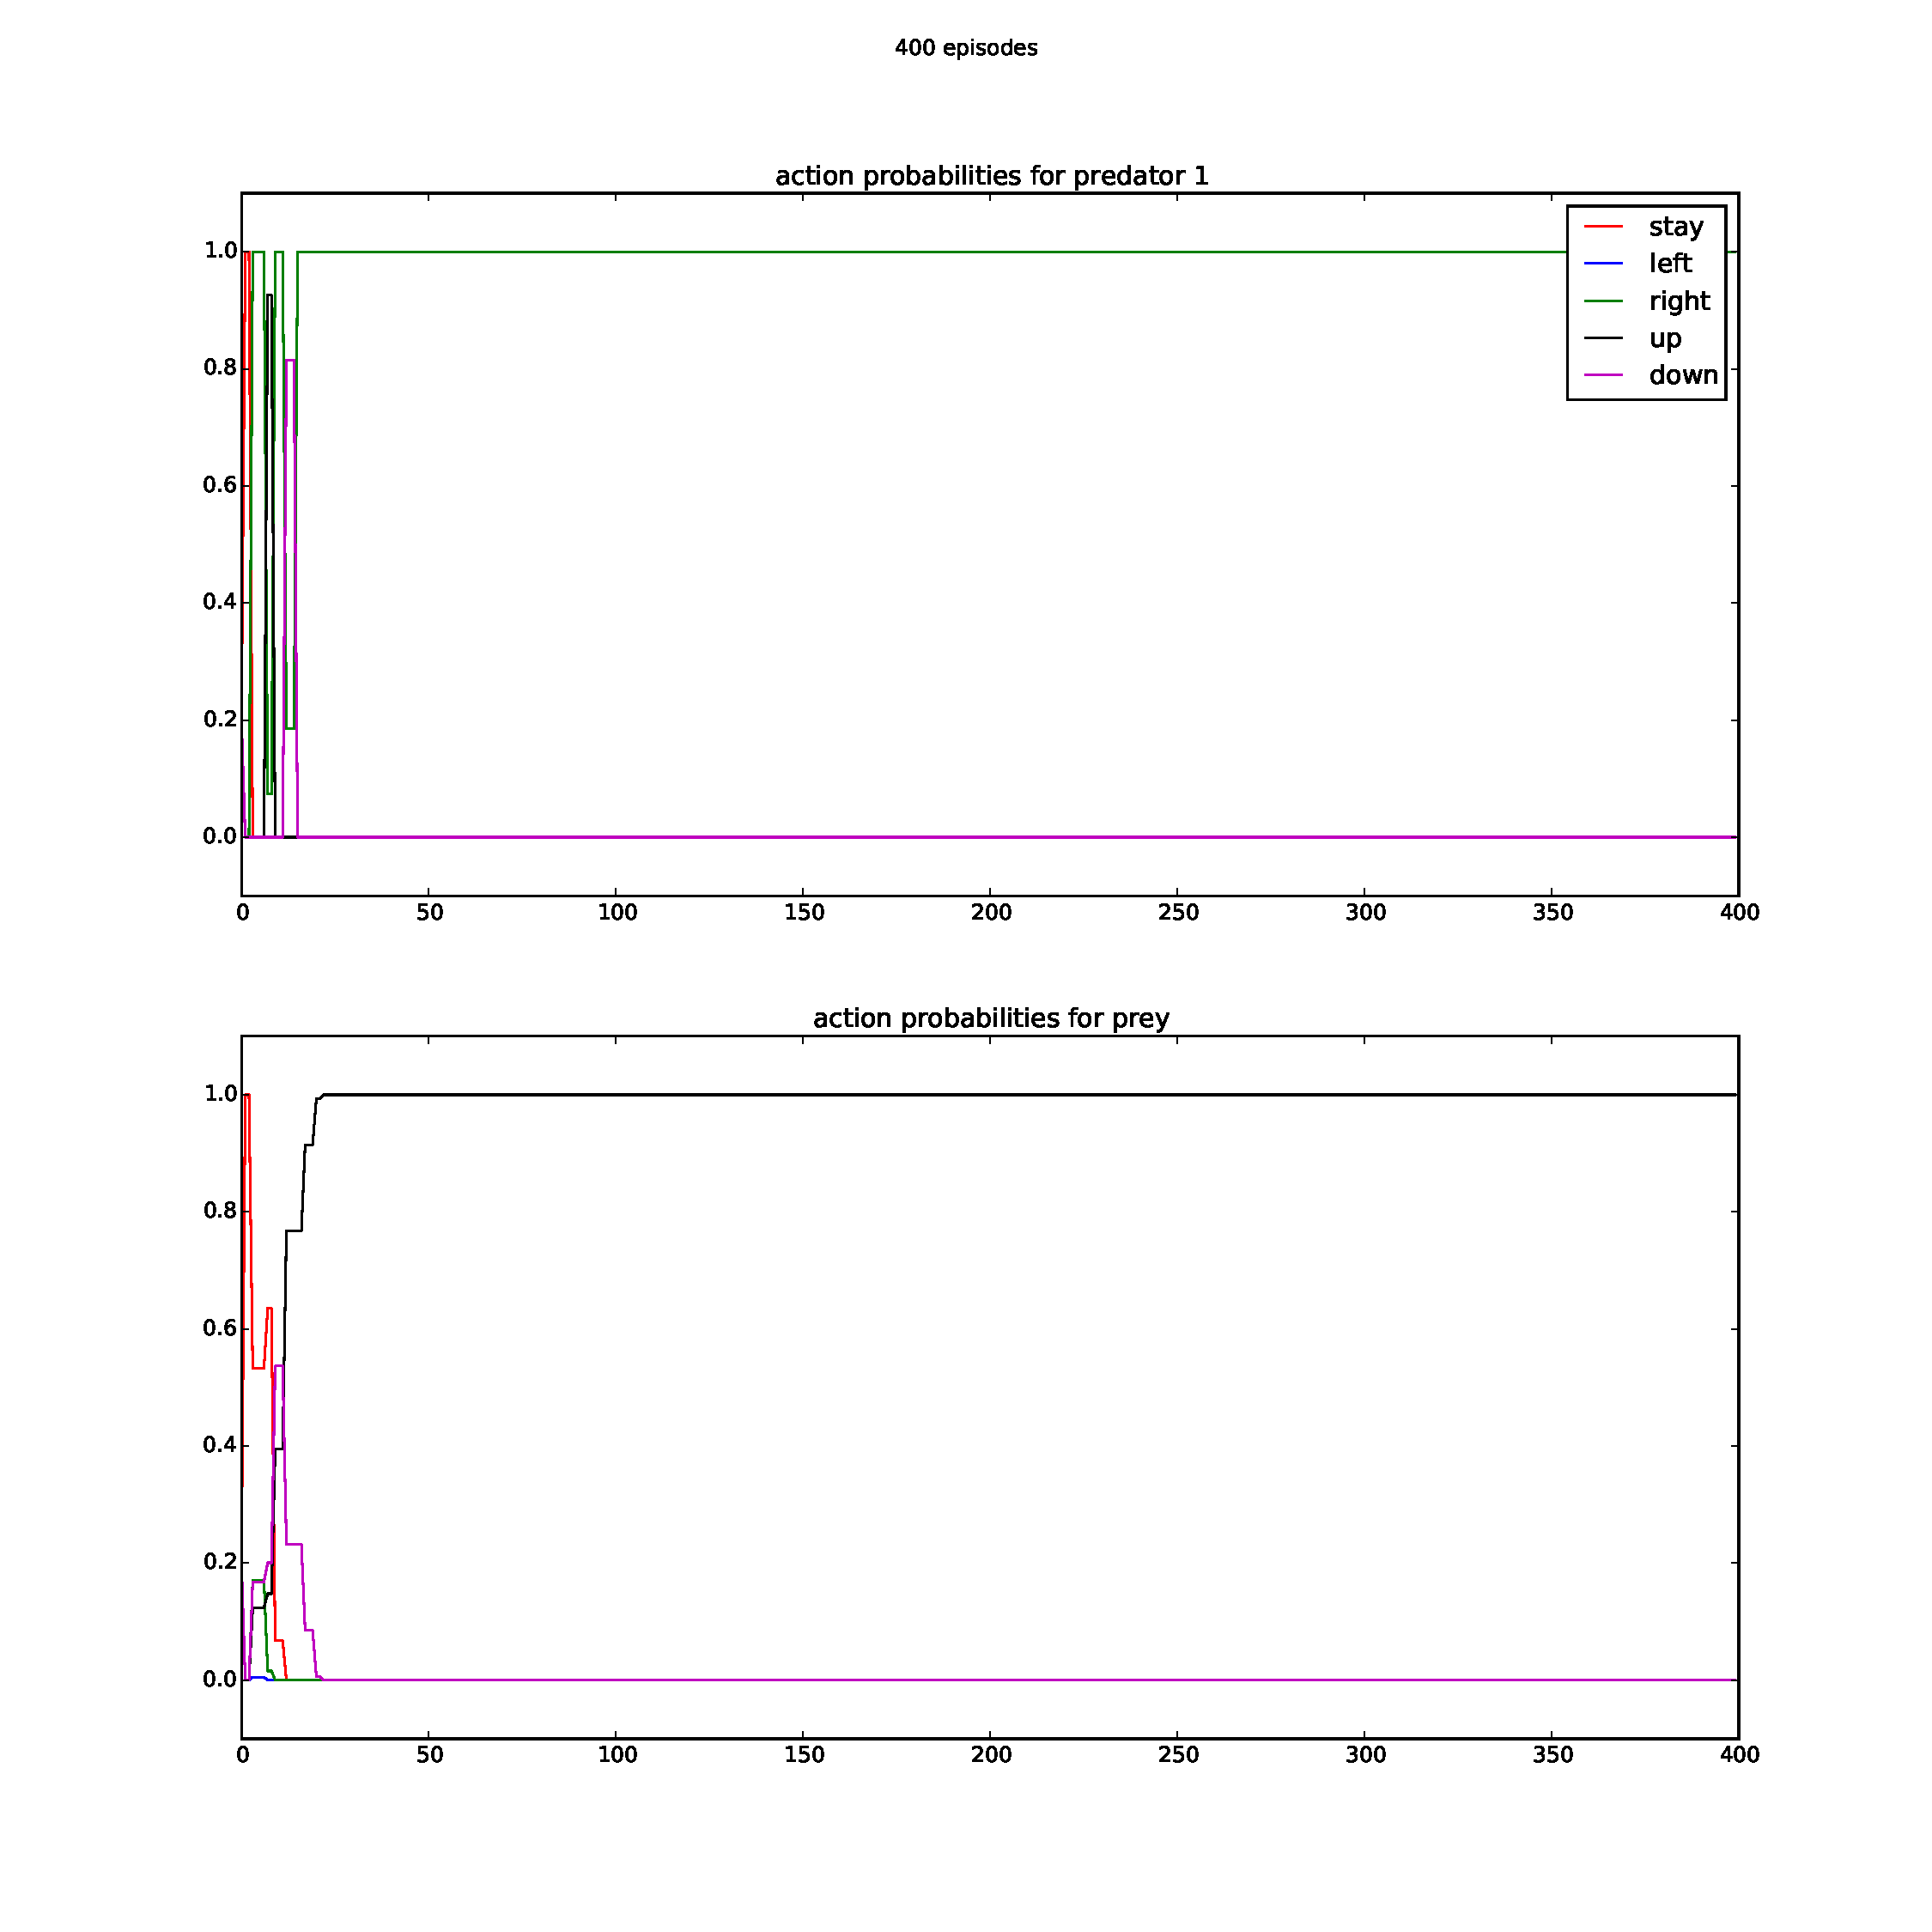
\includegraphics[width=\textwidth]{policychange-minimax-400}
\caption{Convergence of the predator policy to optimal action in Minimax-Q after 25 episodes}
\label{fig:policychange-minimax}
\end{figure}

\subsection{Win-or-Learn-Fast Policy Hill-Climbing (WoLF-PHC)}\label{sec:wolf-phc}

Obviously, independent learning cannot safely converge to an optimal policy because it treats the other agents as part of the environment with a stationary policy, which is not true. As the other agents change their policy, the previously learned best response of our agent may become incorrect. For this reason, a new algorithm called Win-or-Learn-Fast Policy Hill-Climbing (WoLF-PHC) was introduced in \cite{01ijcai-wolf}. It is based on Q-Learning, but     uses two different learning rates for the winning and losing scenario. To determine whether a taken action $a$ in state $s$ was optimal, the policy's expected reward $\sum_a\pi(s,a)Q(s,a)$ is compared to the expected reward of the average policy $\bar{\pi}$. If the first is greater than the latter, the agent learns with the winning stepsize $\delta_w$, otherwise with the losing step-size $\delta_l$, with $\delta_w > \delta_l$. This algorithm retains the rationality of Q-Learning while "encouraging convergence". The implementation of WoLF-PHC can be found in ^wolf\_phc.py^. The policy follows a \textit{mixed strategy}, with $\epsilon$ probability of choosing an exploring action and an additional probability distribution over the optimal actions to prevent exploitation of the strategy by the other agents. This policy can be found in ^Mixed\_policy.py^. In this case, the plearner keeps track of the Q-Values and the ^values^-field inside the policy is used to store the action probabilities for every state. In the paper, WoLF-PHC was shown to converge in multiple experiments.

To visualize the learning progress of the WoLF-PHC algorithm, we set up a 3 by 3 field where in the initial state, the prey sits in the center with two predators to the left and right (fig. \ref{fig:wolfgui}). Then, we run 50'000 episodes and keep track on how the action values change for the three agents in this particular state. The plot in fig. \ref{fig:wolf50k} shows the probability of taking the possible actions in this state. In our experiments, we used a medium-aggresive set of learning rates with $\delta_l=3$ and $\delta_w=1$, that means if the agent is losing, it learns three times faster than when it is winning. Furthermore, a discount factor of $\gamma=0.9$ was used.

As we can see, the first predator will most likely go \textit{right} to the field where the prey resides or \textit{stay} to wait for the move of the prey whereas predator 2 will choose most likely from the \textit{up}, \textit{down} or \textit{stay} actions to counter any potential move of the prey. The prey will try to escape \textit{up} most of the time with a phase where it tries to escape \textit{down} and finally resignates and just sees the \textit{stay} action as the best choice. Since the two predators have a good chance to stay put, this is also the option where the prey has a serious chance of living the longest.

\begin{figure}[h!]
\centering
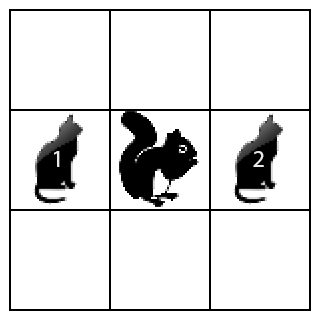
\includegraphics[width=0.3\textwidth]{wolf-gui}
\caption{The state for which the action values are plotted below.}
\label{fig:wolfgui}
\end{figure}


\begin{figure}[h!]
\centering
\includegraphics[width=\textwidth]{policychange-wolf-50000}
\caption{Action values over 50'000 episodes of WoLF-PHC.}
\label{fig:wolf50k}
\end{figure}
\section{Comparison}
In the following experiment we compare a prey with independent Q-learning to a predator with alternatively independent Q-learning, WoLF, SARSA and Softmax in a 5 by 5 grid world.
this comparison is presented in Figure \ref{fig:compalgos}.
It shows the amount of steps the predator takes to catch the prey. The height is the average amount of steps it took in 5 rounds, the x-axis shows the amount of rounds in steps of 5.
The image shows that WoLF performs quite poorly on a q-greedy prey. Sarsa is slightly better but still has high variations. Q-Learning and Softmax both perform quite well with Q-Learning having the edge over Softmax in multiple runs. It seems that countering a Q-Learning prey with Q-Learning is the best approach.

After that, we ran a test to compare the performance if the prey was equipped with a Softmax policy. This can be seen in Figure \ref{fig:compalgos-2}, where you can see that still Q-Learning and Softmax take the lead over WoLF and Sarsa, but Softmax seems to perform a bit better.
In the final comparison we equip the prey with the WoLF learning algorithm. This is shown in Figure \ref{fig:compalgos-3}.
Here WoLF performs poorly against another WoLF but gets beaten by the other algorithms quite quickly.
Our conclusion is that on a small field with two agents, the best algorithms will be the Q-Learning or Softmax algorithms. This might come from the fact that with a tripping chance of 0.2 and only little room to escape, the prey as almost no chance to live up to it's potential with more complex algorithms.

\begin{figure}[h!]
\centering
\includegraphics[width=\textwidth]{different_algos_comp}
\caption{Comparison of different predator algorithms in 300 episodes (shown in steps of 5) - Prey Q-Learning}
\label{fig:compalgos}
\end{figure}

\begin{figure}[h!]
\centering
\includegraphics[width=\textwidth]{different_algos_comp-3}
\caption{Comparison of different predator algorithms in 300 episodes (shown in steps of 5) - Prey Softmax}
\label{fig:compalgos-2}
\end{figure}

\begin{figure}[h!]
\centering
\includegraphics[width=\textwidth]{different_algos_comp-4}
\caption{Comparison of different predator algorithms in 300 episodes (shown in steps of 5) - Prey WoLF}
\label{fig:compalgos-3}
\end{figure}


\newpage
\section{Conclusion}
In this assignment, we explored the various planning/learning algorithms for multi-agent Markov games. We have implemented two naive independent Q-value learning algorithms: independent Q-learning and independent Sarsa. Next we looked at the minimax-Q algorithm, which uses a minimax step to calculate the value and the policy.

For independent Q-learning, we have empirically shown that small learning-rates and high discount factors result in better performance for the predators. We have also shown that Q-learning performs significantly worse when more agents are introduced.

Evaluation of Minimax-Q proved that it converges to the optimal policy, though it is very computationally expensive.

Finally, WoLF Policy Hill Climbing was considered. We have shown how the policies update over the episodes, and can conclude that the agents learn the optimal moves over time.

We conclude that Q-learning performs very well against another Q-learning agent, better than WoLF or Minimax-Q. 
\addcontentsline{toc}{chapter}{\bibname}
\printbibliography 

\end{document}